\documentclass[12pt,a4paper]{article}  
\usepackage[utf8]{inputenc}             
\usepackage{amsmath, amssymb}           
\usepackage{graphicx}                    
\usepackage{geometry}                    
\usepackage{hyperref}   
\usepackage{placeins}                 
\usepackage{tabularx}                    
\geometry{margin=1in}                    

\title{State of the Art: Invasive Glucose Measurement Techniques}
\author{Ahmed Omrani}
\date{\today}

\begin{document}

\maketitle
\tableofcontents
\newpage

%================ Laboratory Plasma Glucose =================%
\section{Laboratory Plasma Glucose Measurement (Gold Standard)}

\subsection{Introduction}
Laboratory plasma glucose measurement represents the \textbf{gold standard} for glucose quantification in clinical and research settings. This method provides highly accurate, precise, and reproducible measurements that are critical for diagnosing diabetes mellitus, monitoring glycemic control in patients, and calibrating other glucose measurement technologies such as Self-Monitoring of Blood Glucose (SMBG) devices and Continuous Glucose Monitoring (CGM) systems \cite{Sacks2011}. Unlike capillary or interstitial measurements, laboratory plasma assays use venous plasma samples, allowing for a controlled environment that minimizes variability due to sample handling, hematocrit, and environmental factors. The method is predominantly enzymatic, using either the hexokinase or glucose oxidase reactions to convert glucose into measurable products. These products are then quantified spectrophotometrically or electrochemically, enabling precise determination of glucose concentration.

\subsection{Historical and Regulatory Context}
The hexokinase method was first introduced in the 1960s and rapidly became the reference method due to its superior specificity, linearity, and minimal interference from substances such as uric acid, ascorbic acid, and other reducing agents present in blood \cite{Hagvik2007}. Earlier methods, including chemical reduction assays like Somogyi-Nelson, lacked specificity and reproducibility, highlighting the need for enzymatic assays in clinical diagnostics. Regulatory agencies such as the Food and Drug Administration (FDA) and the International Organization for Standardization (ISO 15197:2013) mandate the use of reference laboratory methods for validating SMBG and CGM devices \cite{CataChem2020}. Reference laboratories adhere to strict protocols using certified materials, including NIST Standard Reference Material 917 (SRM 917), which ensures inter-laboratory consistency and traceability. This regulatory framework underscores the continued relevance of laboratory plasma glucose measurements, not only for routine diagnostics but also as a benchmark in research studies and device development.

\subsection{Analytical Principles}

\subsubsection{Hexokinase Method}
\FloatBarrier
\begin{figure}[h!]
\centering
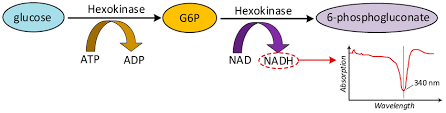
\includegraphics[width=0.8\textwidth]{hexokinase.png}
\caption{Workflow for Laboratory Plasma Glucose Measurement using Hexokinase method.}
\label{fig:hexokinase}
\end{figure}
\FloatBarrier

The hexokinase method is widely recognized for its high specificity and precision. Glucose present in the plasma reacts with adenosine triphosphate (ATP) in the presence of hexokinase to form glucose-6-phosphate (G6P) and adenosine diphosphate (ADP). The G6P then undergoes a second reaction catalyzed by glucose-6-phosphate dehydrogenase (G6PD) in the presence of nicotinamide adenine dinucleotide phosphate (NAD(P)\(^+\)), producing 6-phosphogluconate and NAD(P)H:

\begin{align}
\text{Glucose} + \text{ATP} &\xrightarrow{\text{Hexokinase}} \text{G6P} + \text{ADP} \\
\text{G6P} + \text{NAD(P)}^+ &\xrightarrow{\text{G6PD}} 6\text{-Phosphogluconate} + \text{NAD(P)H}
\end{align}

The amount of NAD(P)H formed is directly proportional to the glucose concentration and can be measured spectrophotometrically at 340 nm \cite{StatPearls2025}. This method offers high reproducibility, minimal interference from other blood constituents, and a broad linear range, making it ideal for both clinical and research applications.

\subsubsection{Glucose Oxidase Method}
The glucose oxidase method catalyzes the oxidation of glucose to gluconolactone, producing hydrogen peroxide as a byproduct:

\[
\text{Glucose} + \text{O}_2 \xrightarrow{\text{Glucose Oxidase}} \text{Gluconolactone} + \text{H}_2\text{O}_2
\]

The hydrogen peroxide generated is quantified either colorimetrically or electrochemically. While this method is widely used in both clinical and point-of-care devices, its accuracy can be affected by oxygen concentration and the presence of other oxidizable substances in plasma \cite{Sacks2011}. Despite these limitations, glucose oxidase remains an essential alternative when spectrophotometric hexokinase assays are not available.

\subsection{Analytical Comparison}
\begin{table}[h!]
\centering
\caption{Comparison of Hexokinase and Glucose Oxidase Methods for Plasma Glucose Measurement}
\begin{tabular}{l c c}
\hline
\textbf{Parameter} & \textbf{Hexokinase} & \textbf{Glucose Oxidase} \\
\hline
Specificity & Very high & Moderate \\
Precision (CV) & $\leq 2.5\%$ & 3--5\% \\
Linear range & 0--600 mg/dL & 5--500 mg/dL \\
Sample volume & 0.5--2 mL & 0.5--2 mL \\
Interference & Minimal & Oxygen, uric acid, ascorbate \\
Measurement time & 5--20 min & 5--25 min \\
Reference traceability & ID-MS & No standardized reference \\
\hline
\end{tabular}
\label{tab:method_comparison}
\end{table}
\noindent
This table summarizes the key analytical parameters, highlighting the superior specificity, precision, and reference traceability of the hexokinase method compared to glucose oxidase. These metrics are critical when selecting a laboratory method for research, clinical diagnostics, or device calibration.

\subsection{Sample Handling and Workflow}
Laboratory plasma glucose measurement requires careful sample handling to ensure accurate results. Blood is drawn via venipuncture into sodium fluoride/oxalate tubes, which inhibit glycolysis. Samples are centrifuged at 3000 rpm for 10 minutes to separate plasma. Immediate analysis is preferred; short-term storage at 4°C is acceptable, but delays can lead to a 5–7\% reduction in glucose concentration per hour \cite{NCBI2023}. Rigorous adherence to sample handling protocols is essential to maintain the integrity of the measurements.

\subsection{Analytical Accuracy and Calibration}
Laboratory analyzers demonstrate high analytical accuracy, with mean bias versus isotope-dilution mass spectrometry (ID-MS) below 1\%. Within-run coefficient of variation (CV) ranges from 1.2–2.0\%, and between-run CV ranges from 1.8–2.5\%. Calibration is performed daily using NIST SRM 917, ensuring consistency and traceability \cite{Sacks2011}.

\subsection{Clinical Interpretation}
Fasting plasma glucose (FPG) is interpreted as normal if $<$100 mg/dL, prediabetic between 100–125 mg/dL, and diabetic $\geq$126 mg/dL. Oral glucose tolerance test (OGTT) and random plasma glucose measurements are also used according to standard clinical guidelines to confirm diabetes diagnosis \cite{StatPearls2025}.

\subsection{Advantages and Limitations}
Laboratory plasma glucose measurement offers unmatched accuracy, specificity, and traceability to reference standards. Its limitations include the invasive nature of venous sampling, the need for laboratory infrastructure, discrete rather than continuous measurements, and critical dependence on proper sample handling.

\subsection{Figures}
\begin{figure}[h!]
\centering
\framebox[0.8\textwidth]{\parbox{0.75\textwidth}{Schematic of Glucose Oxidase Plasma Glucose Measurement Workflow}}
\caption{Laboratory Glucose Oxidase method workflow.}
\label{fig:glucoseoxidase}
\end{figure}

%================ SMBG =================%
\section{Self-Monitoring of Blood Glucose (SMBG)}

\subsection{Introduction}
Self-Monitoring of Blood Glucose empowers patients to measure their blood glucose independently, allowing real-time therapeutic decisions regarding insulin administration, diet, and physical activity. This capability is essential for individuals with type 1 diabetes and insulin-treated type 2 diabetes, where frequent monitoring prevents both hypo- and hyperglycemia. SMBG also provides the opportunity to observe daily glucose trends, enabling patients and clinicians to tailor individualized treatment plans \cite{Bergenstal2017, ADA2025}.

\subsection{Analytical Principles}
SMBG relies on enzymatic electrochemical detection using small volumes of capillary blood, typically 0.3–1 µL obtained via finger-prick. The most common enzymatic reactions are based on glucose oxidase (GOx) or glucose dehydrogenase (GDH):

\[
\text{Glucose} + \text{O}_2 \xrightarrow{\text{Glucose Oxidase}} \text{Gluconolactone} + \text{H}_2\text{O}_2
\]

\[
\text{Glucose} + \text{NAD(P)}^+ \xrightarrow{\text{GDH}} \text{Gluconolactone} + \text{NAD(P)H}
\]

Electrochemical detection of the produced hydrogen peroxide or NAD(P)H provides a signal directly proportional to glucose concentration. Despite the small sample volume, modern SMBG devices offer high accuracy and rapid measurement, making them practical for daily patient use \cite{Heinemann2018}.

\subsection{Accuracy and Regulatory Standards}
ISO 15197:2013 establishes performance standards for SMBG devices, requiring measurements below 100 mg/dL to be within $\pm 15$ mg/dL of reference values, and measurements $\geq 100$ mg/dL within $\pm 15\%$ \cite{ISO15197}. Accuracy can be influenced by hematocrit, environmental conditions, and user technique, underscoring the need for patient education and routine quality control \cite{Heinemann2018}.

\subsection{Clinical Applications}
SMBG is used for insulin dose titration, postprandial glucose monitoring, prevention of hypoglycemia, and trend analysis in combination with CGM data. While SMBG cannot replace laboratory measurements for diagnostic purposes, it is indispensable for daily diabetes management and therapeutic adjustments \cite{ADA2025}.

\subsection{Advantages and Limitations}
SMBG is fast, portable, and minimally invasive, enabling immediate feedback. Limitations include its discrete measurements rather than continuous monitoring, potential discomfort from repeated finger-pricks, and variability due to operator technique or environmental factors.

\subsection{Figure Placeholder}
\begin{figure}[h!]
\centering
\framebox[0.8\textwidth]{\parbox{0.75\textwidth}{SMBG workflow showing finger-prick sampling and electrochemical glucose detection}}
\caption{SMBG workflow.}
\label{fig:smbg_workflow}
\end{figure}

%================ CGM =================%
\section{Continuous Glucose Monitoring (Invasive CGM)}

\subsection{Introduction}
Invasive Continuous Glucose Monitoring (CGM) systems provide dynamic, near real-time monitoring of glucose concentrations in interstitial fluid. By continuously sampling glucose every 1–5 minutes, CGM captures trends and provides alerts for hypo- and hyperglycemia, enhancing glycemic control and reducing the risk of severe glucose excursions \cite{CGM_Ambulatory_Review_2024, CGM_Routine_Care_2024}. CGM complements SMBG by providing continuous data and is increasingly integrated with automated insulin delivery systems.

\subsection{Analytical Principles}
CGM sensors utilize enzymatic electrochemical reactions similar to SMBG, with either glucose oxidase or GDH mediating the oxidation of glucose. The electrochemical signal generated is proportional to glucose concentration. Interstitial glucose measurements lag plasma glucose by 5–10 minutes due to physiological diffusion, which must be considered when interpreting trends \cite{CGM_ICU_Accuracy_2024}.

\subsection{Performance Characteristics}
\FloatBarrier
\begin{table}[h!]
\centering
\caption{Performance of Contemporary CGM Systems (2024--2025)}
\begin{tabularx}{\textwidth}{l X}
\hline
\textbf{Parameter} & \textbf{Value / Range} \\
\hline
Sensor life & 7--14 days \\
Sample medium & Interstitial fluid \\
Measurement frequency & 1--5 minutes \\
MARD & 8--10\% \\
Calibration & Factory-calibrated or twice-daily SMBG \\
Lag time vs plasma glucose & 5--10 minutes \\
Alerts & Customizable for hypo/hyperglycemia \\
Reference traceability & Validated against laboratory plasma glucose and ID-MS \\
\hline
\end{tabularx}
\label{tab:cgm_performance}
\end{table}
\FloatBarrier

\subsection{Analytical Accuracy and Clinical Relevance}
Modern CGM systems achieve a mean absolute relative difference (MARD) of 8–10\% against reference plasma glucose. Sensitivity for detecting hypoglycemia ranges from 85–92\%, and hyperglycemia detection reaches 96–98\%. Continuous alerts allow timely intervention and are instrumental in preventing severe glucose fluctuations \cite{CGM_Routine_Care_2024}.

\subsection{Advantages and Limitations}
CGM offers continuous glucose data, visualization of trends, reduced reliance on SMBG, and integration with insulin delivery systems. Limitations include the 5–10 minute physiological lag, influence of tissue hydration, temperature, and compression, sensor replacement every 7–14 days, and associated costs.

\subsection{Figure Placeholder}
\begin{figure}[h!]
\centering
\framebox[0.8\textwidth]{\parbox{0.75\textwidth}{CGM system schematic showing sensor, transmitter, and receiver workflow}}
\caption{CGM workflow.}
\label{fig:cgm_workflow}
\end{figure}

\subsection{Conclusion}
Invasive glucose measurement techniques, including laboratory plasma glucose, SMBG, and CGM, remain the foundation of diabetes management. Each method provides distinct advantages in terms of accuracy, precision, temporal resolution, and clinical relevance. Together, they support informed clinical decision-making, personalized therapy, and the development and validation of novel glucose monitoring technologies.

\bibliographystyle{ieeetr}
\bibliography{references}

\end{document}